\chapter{State of the Art}
\label{chap:ch2}

\par This chapter outlines the theoretical foundation and current research landscape for the detection of architectural anti-patterns in microservice-based systems.

\section {Microservices Architecture}
\label{section:microservices-background}

\par A collection of loosely coupled services that can be independently deployed, each implementing a specific business requirement, are hereinafter referred to as microservices \cite{Newman2015}. The aforementioned architectural style allows engineers to develop, deploy and scale individual services independently, unlike monolithic architectures, where the entire application is built, tested and deployed as a single unit \cite{Richardson2018}.

Several key principles underpin the microservices architectural style. First, each service should embody a single responsibility, encapsulating a single business domain in accordance with Domain-Driven Design (DDD) \cite{Evans2004}. Closely related is the principle of independent deployability, whereby services can be released without requiring coordinated deployments across the entire system. Furthermore, microservices, advocated for decentralized data management, in which each service owns its data and exposes it only through well-defined APIs, following the database-per-service pattern \cite{Richardson2018}. Communication between services relies on lightweight protocols such as HTTP/REST or asynchronous messaging, avoiding heavyweight middleware. Lastly, fault isolation ensures that failures in one service do not cascade to others, a goal commonly achieved through patterns such as circuit breakers or bulkheads \cite{Nygard2018}.

Figure~\ref{fig:monolith-vs-microservices} demonstrates the fundamental structural distinctions between a monolithic architecture and a microservices architecture. In the monolithic approach, all components reside within a single deployable unit sharing the same database. Conversely, in the microservices approach, each service is independently deployed and manages its own database.

\begin{figure}[htbp]
    \centering
    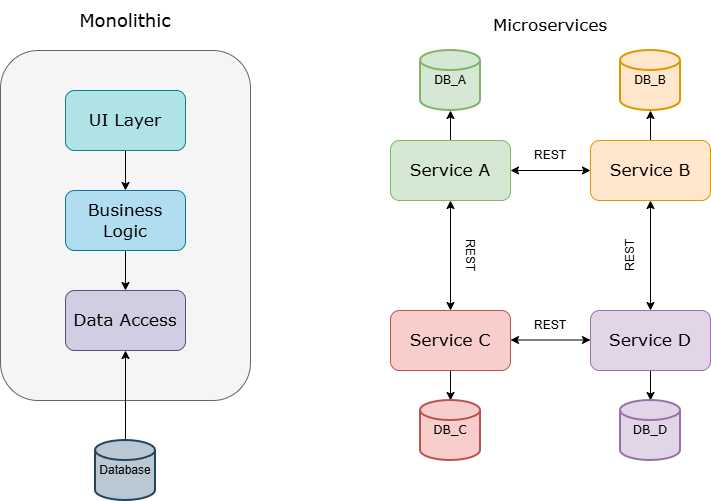
\includegraphics[scale=0.45]{figures/images/chapter2/monolith_vs_microservices.drawio.png}
    \caption{Comparison of monolithic architecture (left) and microservices architecture (right). In the monolithic approach, all modules share a single process and database. In the microservices approach, each service is independently deployable with its own database.}
    \label{fig:monolith-vs-microservices}
\end{figure}

% \textcolor{red}{daca figura e luata de undeva atunci aici in caption pui referinta. Daca iti apartine ca si concept si executie, ignora acest comentariu}

While microservices offer benefits in scalability, team autonomy and technology heterogeneity, they also introduce significant overhead in terms of distributed systems challenges, e.g. network latency, partial failures, data consistency \cite{FowlerMicroservices2014}. When these challenges are poorly managed, they manifest as architectural anti-patterns, i.e. recurring design decisions that negatively impact the quality attributes of the system.

\section{Microservices Anti-Patterns}
\label{sec:anti-patterns}

\par An anti-pattern denotes a frequently used solution to a recurring problem that, rather than resolving it efficiently, introduces a set of negative consequences that may exacerbate the issue further \cite{Brown1998}. In the context of microservices, anti-patterns represent architectural or design decisions that undermine the benefits of the microservices pattern. This section defines and characterizes the anti-patterns targeted by this dissertation, whereas the specific implementation details are presented in Chapter~\ref{chap:ch3}.

\subsection{Shared Database}
\label{subsec:shared-database}

\par The Shared Database anti-pattern occurs when multiple microservices are allowed access to modify the same database schema, which is a violation of the principle of decentralized data management \cite{Richardson2018}. This creates tight coupling between services at the data layer, as changes to the database schema can break multiple services simultaneously. Furthermore, services cannot be independently deployed or scaled without considering the shared database.

As illustrated in Figure~\ref{fig:shared-database}, when services A, B and C all connect to the same database, any schema migration in one service can cause failures in the other. The recommended remediation is to adopt the database-per-service pattern and synchronize data across services using asynchronous events or the Saga pattern \cite{Richardson2018}.

\begin{figure}[htbp]
    \centering
    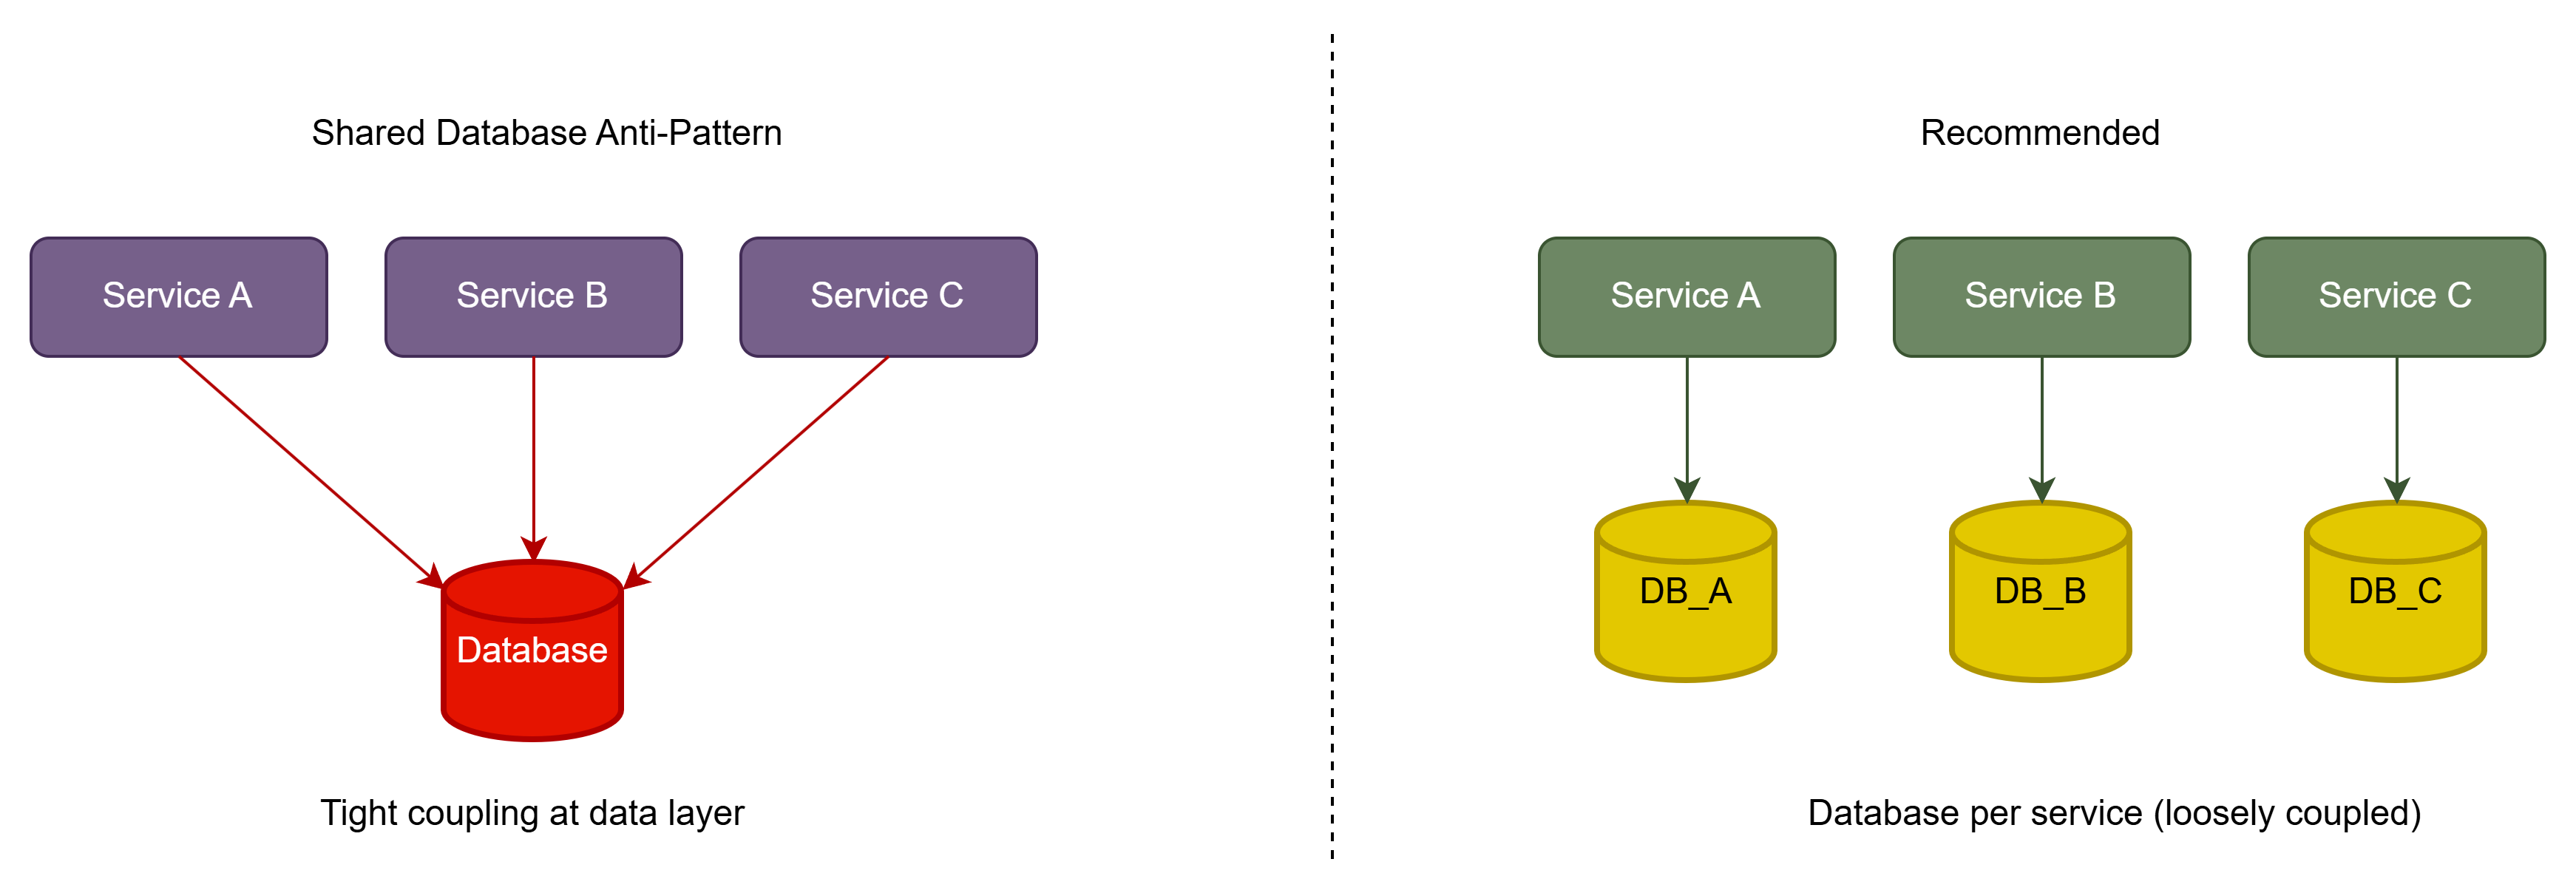
\includegraphics[scale=0.10]{figures/images/chapter2/shared_db.drawio.png}
    \caption{Shared Database Anti-Pattern: multiple services access the same database instance, creating tight coupling at the data layer.}
    \label{fig:shared-database}
\end{figure}

% The concretestatic detection method used for this anti-pattern is presented in Chapter~\ref{chap:ch3}, Section~\ref{subsec:detect-shared-database}.

\subsection{Cyclic Dependency}
\label{subsec:cyclic-dependency}

\par Cyclic dependencies occur when two or more services form a circular chain of dependencies (e.g., in an online shopping application, the Order Service depends on the Payment Service, which depends on the Inventory Service, which in turn depends back on the Order Service, forming a circular dependency). Cycles in the service dependency graph violate the acyclic dependencies principle and create tight coupling, making it fairly difficult to deploy, test, or reason about services independently \cite{Martin2017}.

% The concretegraph-based detection method used for this anti-pattern is presented in Chapter~\ref{chap:ch3}, Section~\ref{subsec:detect-cyclic-dependency}.

Figure~\ref{fig:cyclic-dependency} illustrates a cyclic dependency among three services, as presented in the introduction of this subsection.

\begin{figure}[htbp]
    \centering
    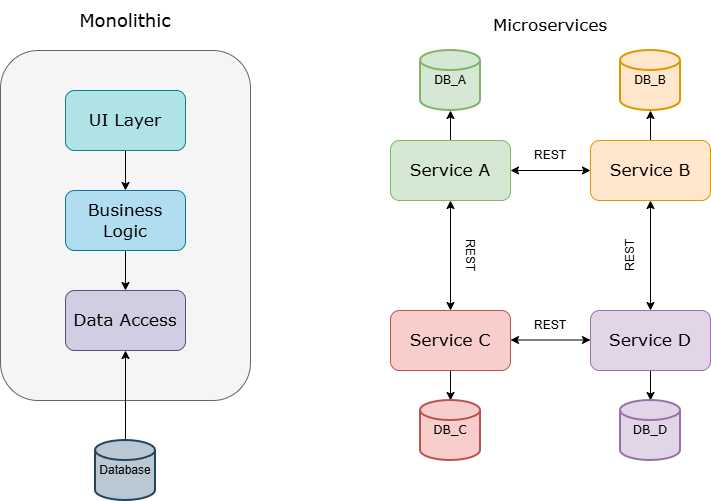
\includegraphics[scale=0.15]{figures/images/chapter2/cyclic-dependency.drawio.png}
    \caption{Example of a cyclic dependency. Services A, B and C form a strongly connected component where no service can be deployed or tested independently.}
    \label{fig:cyclic-dependency}
\end{figure}

\subsection{Nano Service}
\label{subsec:nano-service}

\par A service that is too fine-grained to justify its operational overhead is referred to in this work as a Nano Service, following microservice anti-pattern catalogues that describe nano services as the result of overly fine-grained decomposition \cite{Tighilt2023}. This concern is closely related to the Microservice Greedy smell reported by Taibi and Lenarduzzi, where teams create new microservices even when the resulting services provide very limited functionality \cite{Taibi2018}. Each microservice carries inherent costs: monitoring, deployment pipelines, network communication, and operational maintenance. When a service has very few lines of code and exposes only one or two endpoints, the overhead of running it as an independent process may outweigh the benefits of decomposition.

% The concretethreshold-based detection method used for this anti-pattern is presented in Chapter~\ref{chap:ch3}, Section~\ref{subsec:detect-nano-service}.

The recommended remediation for nano services is to reconsider the service boundary and, when separate deployment is not justified, merge the service with a related, functionally cohesive service \cite{Tighilt2023}.

\subsection{God Service}
\label{subsec:god-service}

\par A God Service is the microservice counterpart of the well-known God Class code smell, also documented as the ''Blob'' anti-pattern \cite{Brown1998}. It refers to a service that handles too many responsibilities, spanning multiple business domains within a single deployable unit. God services grow over time as developers add functionality to an existing service rather than creating new ones, resulting in a service that is difficult to understand, test, and scale independently.

% The concretestructural detection method used for this anti-pattern is presented in Chapter~\ref{chap:ch3}, Section~\ref{subsec:detect-god-service}.

\subsection{Chatty Service}
\label{subsec:chatty-service}

\par The Chatty Service anti-pattern occurs when a service makes an excessive number of fine-grained remote calls to another service to complete a single business operation \cite{Richardson2018}. This increases network latency, reduces throughput, and makes the system fragile to network failures. The chatty communication pattern often indicates that the service boundaries were drawn incorrectly, and data that should be co-located is split across services.

% The concretedetection method used for this anti-pattern is presented in Chapter~\ref{chap:ch3}, Section~\ref{subsec:detect-chatty-service}.

Figure~\ref{fig:chatty-services} contrasts a chatty communication pattern with a well-designed coarse-grained interaction. In the chatty pattern, Service A makes many fine-grained calls to Service B to complete a single operation, whereas the improved design consolidates these into fewer, coarser-grained requests.

\begin{figure}[htbp]
    \centering
    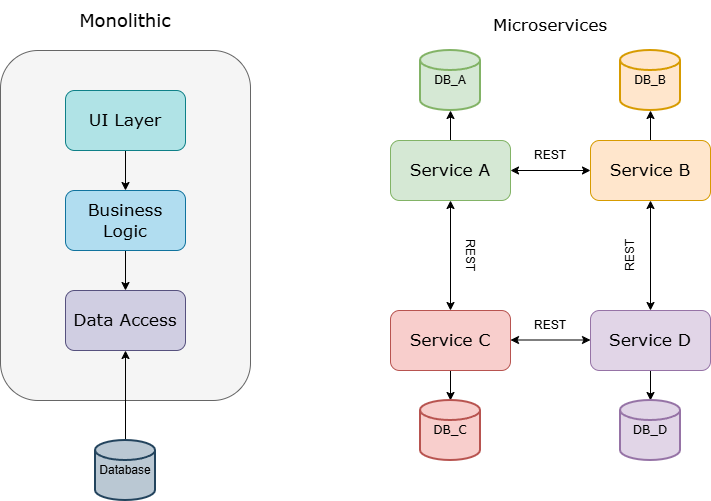
\includegraphics[scale=0.08]{figures/images/chapter2/chatty-services.drawio.png}
    \caption{Example of chatty services versus coarse-grained services. Chatty Service A sends too many requests to Service B, whereas Coarse-Grained Service A sends fewer, more consolidated requests.}
    \label{fig:chatty-services}
\end{figure}

\subsection{Hardcoded Endpoints}
\label{subsec:hardcoded-endpoints}

\par The Hardcoded Endpoints anti-pattern occurs when service URLs are embedded directly in the source code instead of being resolved through a service discovery mechanism (e.g., Netflix Eureka, Consul, or Kubernetes DNS) \cite{Richardson2018}. Hardcoded endpoints create tight coupling between services and make the system inflexible to infrastructure changes such as scaling, failover, or environment migration.

% The concretesource-code detection method used for this anti-pattern is presented in Chapter~\ref{chap:ch3}, Section~\ref{subsec:detect-hardcoded-endpoint}.

\subsection{Distributed Monolith}
\label{subsec:distributed-monolith}

\par The Distributed Monolith anti-pattern describes a system that has been decomposed into multiple services but retains the tight coupling characteristics of a monolithic architecture \cite{Newman2015}. In such a system, services cannot be deployed, tested, or scaled independently, as a change in one service frequently requires coordinated changes and redeployments across several other services. The result is a system that combines the complexity of distributed systems (network latency, partial failures, operational overhead) with none of the benefits of microservices (independent deployability, team autonomy, technology heterogeneity).

A distributed monolith typically arises when services share too many dependencies, communicate excessively, or rely on synchronous call chains to fulfill requests.

% The concretemetric-based detection method used for this anti-pattern is presented in Chapter~\ref{chap:ch3}, Section~\ref{subsec:detect-distributed-monolith}.

The recommended remediation involves identifying and removing unnecessary inter-service dependencies, introducing asynchronous communication where possible, and ensuring that each service encapsulates a well-defined bounded context with minimal external dependencies \cite{Richardson2018}.

\subsection{Additional Anti-Patterns}
\label{subsec:anti-patterns-summary}

\par Beyond the primary anti-patterns described in the preceding subsections, this work targets three additional anti-patterns that address gaps in API governance, service boundary design, and communication topology.

\par API Versioning Absence occurs when services expose REST endpoints without a versioning strategy (e.g.\ a \texttt{/v1/} path prefix), making it harder to introduce breaking API changes while preserving compatibility for existing consumers \cite{Taibi2018, Walker2020}. In rapidly evolving microservice systems, the absence of versioning can force coordinated deployments across consumer services whenever an endpoint's contract changes, undermining the independent deployability that microservices are designed to provide.

% The concretedetection method used for this anti-pattern is presented in Chapter~\ref{chap:ch3}, Section~\ref{subsec:detect-versioning-absence}.

\par Wrong Cuts refers to service boundaries that do not align with business domain boundaries, resulting in high coupling and low cohesion across services \cite{Taibi2018}. When functionality that belongs to a single bounded context is split across multiple services, the resulting inter-service communication overhead and tight coupling negate the benefits of decomposition.

% The concretedetection method used for this anti-pattern is presented in Chapter~\ref{chap:ch3}, Section~\ref{subsec:detect-wrong-cuts}.

\par ESB Misuse occurs when a single service mediates most inter-service communication, effectively recreating the Enterprise Service Bus pattern within a microservices architecture \cite{Richards2015}. This centralisation introduces a single point of failure, a performance bottleneck, and a deployment coupling point that contradicts the decentralised communication principle of microservices.

% The concretedetection method used for this anti-pattern is presented in Chapter~\ref{chap:ch3}, Section~\ref{subsec:detect-esb-misuse}.

Table~\ref{tab:anti-patterns-summary} summarizes all the anti-patterns targeted by this dissertation, along with their severity levels and the Chapter~\ref{chap:ch3} sections that describe their detection methodology.

\begin{table}[!ht]
    \begin{center}
        \begin{tabular}{|l|l|p{180pt}|}
            \hline
            \textbf{Anti-Pattern} & \textbf{Severity} & \textbf{Detection Methodology} \\
            \hline\hline
            Shared Database & High & Section~\ref{subsec:detect-shared-database} \\
            \hline
            Cyclic Dependency & Critical & Section~\ref{subsec:detect-cyclic-dependency} \\
            \hline
            Nano Service & Medium & Section~\ref{subsec:detect-nano-service} \\
            \hline
            God Service & High & Section~\ref{subsec:detect-god-service} \\
            \hline
            Chatty Service & High & Section~\ref{subsec:detect-chatty-service} \\
            \hline
            Hardcoded Endpoints & Medium & Section~\ref{subsec:detect-hardcoded-endpoint} \\
            \hline
            Distributed Monolith & Critical & Section~\ref{subsec:detect-distributed-monolith} \\
            \hline
            API Versioning Absence & Medium & Section~\ref{subsec:detect-versioning-absence} \\
            \hline
            Wrong Cuts & High & Section~\ref{subsec:detect-wrong-cuts} \\
            \hline
            ESB Misuse & High & Section~\ref{subsec:detect-esb-misuse} \\
            \hline
        \end{tabular}
    \end{center}
    \caption{Summary of targeted microservice anti-patterns and references to their detection methodology.}
    \label{tab:anti-patterns-summary}
\end{table}

\section{Related Work}
\label{sec:related-work}

\par The detection of anti-patterns in microservices architectures has received growing attention from the scientific research community. This section reviews the most relevant prior work and positions this dissertation within the existing landscape.

\subsection{Systematic Reviews and Grey Literature Studies}
\label{subsec:systematic-reviews}

\par Several systematic literature reviews have mapped the state of research on microservices, providing a broad understanding of the field's maturity and open challenges.

Di-Francesco et al.\ conducted a systematic mapping study on research related to microservices architecture, analyzing 71 studies published between 2014 and 2016 \cite{DiFrancesco2017}. Their findings revealed that the majority of research focused on migration from monolithic to microservice architectures, with comparatively little attention to quality assurance, anti-pattern detection, and automated analysis tools. The authors identified an appreciable gap between the industrial adoption of microservices and the availability of rigorous academic research that addresses the architectural challenges that practitioners face. This gap motivates the need for tools that can aid development teams in identifying architectural debt in microservice systems.

Soldani et al.\ performed a systematic grey literature review covering 51 industrial experience reports and practitioner blog posts on microservices \cite{Soldani2018}. Their study identified the most frequently reported pains (challenges) and gains (benefits) of microservice adoption. Among the pains, the most commonly reported were increased complexity in distributed systems, difficulties with data management across services, and challenges related to monitoring and debugging. Notably, several of the anti-patterns targeted by this dissertation correspond to the pains reported by the practitioners in the aforementioned study: the Shared Database anti-pattern relates to data management difficulties, the Distributed Monolith corresponds to accidental tight coupling, and the Chatty Service pattern reflects the complexity of managing inter-service communication. The alignment between practitioner-reported challenges and the anti-patterns detected by this work supports its relevance.

\subsection{Empirical Studies on Microservices Anti-Patterns}
\label{subsec:empirical-studies}

\par Taibi and Lenarduzzi conducted an empirical study involving interviews with 72 experienced developers, identifying the most common "bad smells" in microservice architectures \cite{Taibi2018}. Their findings highlighted that Wrong Cuts, Shared Database (also referred to as "Shared Persistency") and Hardcoded Endpoints are among the most frequently encountered and impactful anti-patterns in enterprise practice. The study also reported that many teams were unaware of these anti-patterns until they had accumulated enough significant technical debt, underscoring the value of automated detection tools. This empirical evidence informed the selection of anti-patterns targeted by this dissertation.

In a subsequent work, Taibi, Lenarduzzi, and Pahl proposed a structured taxonomy that catalogues twenty microservice anti-patterns grouped into \emph{technical} and \emph{organizational} categories, each further divided into subcategories, i.e. internal and communication smells on the technical side, and team-oriented and technology/tool-oriented smells on the organizational side \cite{Taibi2020}. This taxonomy provides a principled framework for reasoning about the origins of microservice anti-patterns. Drawing on this and the broader anti-pattern literature, the present dissertation organizes the ten anti-patterns it targets into four architectural dimensions of its own, i.e. service design, communication, data management, and deployment and coupling, as summarized in Table~\ref{tab:antipattern-dimensions}.

\begin{table}[htbp]
    \begin{center}
        \small
        \begin{tabular}{|l|l|p{170pt}|}
            \hline
            \textbf{Architectural Dimension} & \textbf{Anti-Pattern} & \textbf{Concern Addressed} \\
            \hline\hline
            \multirow{2}{*}{Service Design}
            & Nano Service   & Service too small to justify operational overhead \\
            \cline{2-3}
            & God Service    & Service handling too many responsibilities \\
            \hline
            \multirow{4}{*}{Communication}
            & Chatty Service       & Excessive fine-grained inter-service calls \\
            \cline{2-3}
            & Cyclic Dependency    & Circular dependency chains between services \\
            \cline{2-3}
            & ESB Misuse           & Single service mediating most communication \\
            \cline{2-3}
            & Hardcoded Endpoints  & Service URLs hardcoded instead of using discovery \\
            \hline
            Data Management
            & Shared Database      & Multiple services accessing the same database \\
            \hline
            \multirow{3}{*}{Deployment \& Coupling}
            & Distributed Monolith    & Tightly coupled services requiring co-deployment \\
            \cline{2-3}
            & Wrong Cuts              & Misplaced service boundaries causing high coupling \\
            \cline{2-3}
            & API Versioning Absence  & No API versioning strategy detected \\
            \hline
        \end{tabular}
    \end{center}
    \caption{Mapping of the ten anti-patterns detected by this work to four architectural dimensions. The grouping is the author's own, inspired by the microservice anti-pattern literature \cite{Taibi2018, Taibi2020}.}
    \label{tab:antipattern-dimensions}
\end{table}

Bogner et al.\ conducted a literature review investigating maintainability measurement for service- and microservice-based systems \cite{Bogner2019}. They mapped candidate metrics to four dominant design properties, i.e.\ size, complexity, coupling and cohesion, and argued that microservice-specific factors such as many services, technological heterogeneity and decentralised control make automatic metric collection difficult without specialised tool support. This observation aligns with a notable contribution of this dissertation: combining intra-service code smell detection with inter-service dependency analysis to provide a panoramic assessment of architectural quality.

\subsection{Static Analysis Approaches}
\label{subsec:related-static}

\par Neri et al.\ conducted a multivocal review of microservice design principles and the architectural smells that violate them \cite{Neri2020}. Their work catalogued seven architectural smells, framed as violations of design principles such as service autonomy, decentralized data management, and smart endpoints and dumb pipes, together with sixteen refactorings to resolve them. While their work provides a strong principled foundation for reasoning about microservice quality, it does not integrate code-level smell detection into the architectural analysis and does not provide an implemented tool with configurable thresholds.

Sharma and Spinellis provided a comprehensive survey on software smells and demonstrated the role of automated tools in detecting them \cite{Sharma2018}. DesigniteJava, presented as a large-scale multi-faceted code smell detection tool by Sharma \cite{Sharma2024}, detects code smells and computes object-oriented metrics for Java projects. While DesigniteJava operates at code level within individual projects, this dissertation uses the aggregate density of these smells as the code-quality signal that contributes to the composite health score, complementing the architectural-level analysis carried out through Spoon-based structural metrics and dependency-graph algorithms.

Pigazzini et al.\ proposed an approach for detecting microservice smells by combining structural analysis with dependency extraction \cite{Pigazzini2020}. Their work focused on identifying smells such as Cyclic Dependencies, Hardcoded Endpoints, and Shared Persistence by analyzing dependency structure extracted from Docker and Spring configuration files (\texttt{docker-compose.yml}, \texttt{Dockerfile}, \texttt{application.yml}) together with source-code communication patterns such as Feign and \texttt{RestTemplate} usage. While their approach addresses inter-service structural smells, it does not incorporate intra-service code smell analysis and does not support the breadth of anti-patterns covered by this dissertation.

Cerny et al.\ provided a contextual analysis of microservice architecture, surveying current research directions and identifying gaps in automated analysis capabilities \cite{Cerny2018}. They highlighted the need for tools that can automatically reconstruct microservice architectures from source code and detect anti-patterns without requiring manual configuration. The automated microservice detection mechanism implemented in this work directly addresses this need by scanning for build files and applying a deployability gate to identify service boundaries without manual configuration.

\subsection{Dynamic and Hybrid Approaches}
\label{subsec:related-dynamic}

\par Dynamic analysis approaches monitor running systems to detect anti-patterns from runtime behaviour. Distributed tracing tools such as Jaeger or Zipkin can reveal chatty communication patterns and cyclic call chains at runtime by recording the flow of requests across service boundaries. However, dynamic approaches require a running system with representative workloads and instrumented services, making them less suitable for early-stage analysis, code review workflows, or integration into CI/CD pipelines where the system is not deployed.

Hybrid approaches combine static and dynamic analysis. For instance, a tool might perform static dependency extraction from source code and complement it with runtime call frequency data collected via distributed tracing. While hybrid approaches can provide higher accuracy (e.g. by confirming the a statically detected dependency is actually exercised at runtime), they introduce additional complexity and infrastructure requirements. They also require the system to be deployed and exercised with representative traffic, which is not always feasible.

This dissertation focuses on static analysis to enable anti-pattern detection without requiring a running system, making it applicable to source repositories at any stage of development. This design choice prioritizes broad applicability and ease of integration over the higher precision that runtime data could provide.

\subsection{Automated Detection Tools}
\label{subsec:related-tools}

\par Several tools have been developed for microservice analysis. This subsection reviews the most relevant ones and highlights their strengths and limitations relative to this work.

\par Arcan serves as a tool developed for detection and analysis of architectural smells in Java projects that supports dependency graph analysis and cycle detection \cite{Arcelli2017}. It detects architectural smells such as Cyclic Dependencies and Unstable Dependencies by constructing and analyzing a dependency graph from compiled Java bytecode. However, Arcan was primarily designed with monolithic Java applications in mind and does not specifically target microservice anti-patterns such as Shared Database (or Persistence), Chatty Service or Distributed Monolith. It also does not provide automated microservice boundary detection or a composite health score.

\par MicroART recovers the architecture of microservice-based systems by combining static information from the source repository with dynamic analysis of the running system \cite{Granchelli2017}. It clones the project's repository to extract service metadata and then monitors the deployed containers at runtime, querying the Docker runtime and capturing inter-service network traffic to reconstruct the actual service interactions, which an architect can subsequently refine. While MicroART does address the important problem of architecture recovery, it focuses on visualization rather than anti-pattern detection. It does not analyze source code for code smells, does not compute coupling metrics and does not provide remediation recommendations.

\par MSANose is a detection tool specifically designed for microservice smells, based on the catalog established by Taibi et al.\ \cite{Walker2020}. It detects smells such as Shared Database, Cyclic Dependencies, Hardcoded Endpoints, ESB Usage, Wrong Cuts, API Versioning, and Microservice Greedy through static analysis for Java-based microservice projects. MSANose represents one close prior work to this dissertation, particularly among static Java-based microservice smell detectors. However, it differs in several respects: it does not integrate a general intra-service code-level smell catalogue into the architectural assessment, it does not compute a composite health score, and it does not target God Service or Chatty Service as defined and implemented in this dissertation.

\par MARS, proposed by Tighilt et al., is a tool-supported approach for specifying and detecting microservice anti-patterns through source-code analysis \cite{Tighilt2023}. It targets sixteen microservice anti-patterns and was empirically validated on 24 microservice-based systems, reporting an average precision of 82\% and recall of 89\%. MARS therefore provides broader anti-pattern coverage than this dissertation. The contribution of the present work is positioned differently: it focuses on a selected set of ten anti-patterns and combines their detection with DesigniteJava-based intra-service smell density, Spoon-based structural metrics, a composite architectural health score, evidence snippets, remediation guidance, analysis history, and a web/API workflow for Java Spring Boot projects.

% Table~\ref{tab:related-tools-comparison} provides a detailed feature comparison of these tools against the system presented in this dissertation.
%
% \begin{table}[htbp]
%     \begin{center}
%         \small
%         \begin{tabular}{|p{100pt}|c|c|c|c|}
%             \hline
%             \textbf{Feature} & \textbf{Arcan} & \textbf{MicroART} & \textbf{MSANose} & \textbf{This Work} \\
%             \hline\hline
%             Targets microservices & $\times$ & \checkmark & \checkmark & \checkmark \\
%             \hline
%             General intra-service code smell detection & \checkmark & $\times$ & Partial & \checkmark \\
%             \hline
%             Cycle detection & \checkmark & $\times$ & \checkmark & \checkmark \\
%             \hline
%             Shared database detection & $\times$ & $\times$ & \checkmark & \checkmark \\
%             \hline
%             God service detection & $\times$ & $\times$ & $\times$ & \checkmark \\
%             \hline
%             Chatty service detection & $\times$ & $\times$ & $\times$ & \checkmark \\
%             \hline
%             Hardcoded endpoints & $\times$ & $\times$ & \checkmark & \checkmark \\
%             \hline
%             ESB misuse detection & $\times$ & $\times$ & \checkmark & \checkmark \\
%             \hline
%             Wrong cuts detection & $\times$ & $\times$ & \checkmark & \checkmark \\
%             \hline
%             API versioning check & $\times$ & $\times$ & \checkmark & \checkmark \\
%             \hline
%             Auto service discovery & $\times$ & Partial & $\times$ & \checkmark \\
%             \hline
%             Health score metric & $\times$ & $\times$ & $\times$ & \checkmark \\
%             \hline
%             Web interface / API & $\times$ & \checkmark & $\times$ & \checkmark \\
%             \hline
%             Configurable thresholds & $\times$ & $\times$ & Partial & \checkmark \\
%             \hline
%             Code snippet evidence & $\times$ & $\times$ & $\times$ & \checkmark \\
%             \hline
%             Remediation guidance & $\times$ & $\times$ & $\times$ & \checkmark \\
%             \hline
%             Target language & Java & Multi & Java & Java \\
%             \hline
%             Analysis technique & Static & Hybrid & Static & Static \\
%             \hline
%         \end{tabular}
%     \end{center}
%     \caption{Feature comparison of related architectural analysis tools. \checkmark\ indicates the feature is supported, $\times$\ indicates it is not supported. ''Partial'' indicates limited support. For MSANose, ''Partial'' in the intra-service code-smell row means it detects microservice-specific smells but does not integrate a general intra-service smell catalogue such as DesigniteJava or use smell density as a health-score dimension; ''Partial'' in the configurable-thresholds row reflects that it exposes only a single adjustable ESB connectivity threshold rather than broadly externalized configuration.}
%     \label{tab:related-tools-comparison}
% \end{table}

\subsection{Positioning and Contributions of This Work}
\label{subsec:positioning}

\par This dissertation differentiates itself from existing work in several ways, addressing gaps identified in the reviewed literature.

First, this work performs multi-level analysis. Existing tools typically operate at a single level of abstraction: either code-level smell detection (e.g.\ DesigniteJava) or architectural-level dependency analysis (e.g.\ Arcan, MicroART). This work combines intra-service code analysis, comprising DesigniteJava smell density together with Spoon-based structural metrics, with inter-service architectural analysis via graph algorithms, providing a more comprehensive assessment. For example, code-level structural metrics such as class cohesion, computed via Spoon, are used as evidence for flagging god services at the architectural level.

Second, the tool offers coverage across several architectural dimensions, detecting ten selected anti-patterns: service design (Nano Service, God Service), inter-service communication (Chatty Service, Cyclic Dependency, Hardcoded Endpoints, ESB misuse), data management (Shared Database), and system-level coupling (Distributed Monolith, API Versioning Absence, Wrong Cuts). Although MARS covers a larger catalogue of anti-patterns, this work emphasizes the integration of selected service-level and system-level findings with code-level smell evidence, configurable thresholds, evidence snippets, remediation guidance, and a composite health score.

Third, the tool provides automated microservice detection by automatically identifying microservice boundaries within a multi-module project. Candidate modules are first discovered by scanning for build files (\texttt{pom.xml}, \texttt{build.gradle}, \texttt{build.gradle.kts}) and are then filtered through a \textit{deployability gate} that verifies whether each candidate is an independently deployable service using three signals applied in priority order: a framework entry point (e.g.\ \texttt{@SpringBootApplication}), the presence of a Dockerfile, or a \texttt{main()} method. This eliminates the need for manual service enumeration, which is required by most existing tools. Multi-module Maven and Gradle projects are supported, with automatic filtering of non-service modules (e.g.\ examples, tests, build support) and parent aggregator modules.

Fourth, detection thresholds for metrics-based anti-patterns are externalized as configurable detection parameters (via Spring Boot's \texttt{application.yml}), allowing calibration to project-specific norms. For instance, the LOC threshold for nano service detection or the call count threshold for chatty service detection can be adjusted without modifying the source code.

Fifth, a composite health score provides a single numeric metric (0-100) for architectural quality, accompanied by a letter grade (A through F). Unlike a simple aggregate, the score is decomposed into four weighted categories, anti-pattern severity, code quality, architectural coupling, and service sizing, each with an itemized list of deductions. Because each deduction is attributed to a specific finding within one of these categories, a low score can be traced back to the dimension that caused it rather than read as a single opaque number, and the per-category scores can be compared across successive analysis runs.

Sixth, unlike existing tools that report anti-patterns as abstract findings, this work supports evidence-based reporting with code snippets attached to each detected anti-pattern. When a cyclic dependency is detected, the tool extracts and presents the relevant \texttt{@FeignClient} annotation or \texttt{RestTemplate} invocation from the source code, providing developers with immediate context for understanding and remediating the issue.

Finally, the tool is delivered as a web application with a RESTful API, supporting both interactive use through a web dashboard and programmatic integration into CI/CD pipelines for continuous architectural quality monitoring. Users can submit projects for analysis either by uploading a ZIP archive or by providing a Git repository URL, which is cloned automatically via JGit.

\section{Summary}
\label{sec:summary}

\par This chapter has established the theoretical and related-work foundation for this dissertation. The microservices architectural style was introduced along its core principles, inherent challenges and a taxonomy of ten microservice anti-patterns.

The related work was reviewed across four categories: systematic literature reviews that map the research landscape, empirical studies that identify practitioner-reported anti-patterns, static analysis approaches that formalize detection techniques, and automated tools that implement detection. The review revealed that existing tools tend to operate at a single level of abstraction or focus on particular subsets of architectural concerns. This dissertation addresses these gaps by combining intra-service and inter-service analysis, supporting ten anti-patterns across four architectural dimensions, providing automated microservice detection, configurable thresholds, evidence-based reporting with code snippets, and a category-based composite health score with letter grading for tracking architectural quality over time. The next chapter presents the detailed detection methodology for each anti-pattern.
